
\documentclass[preprint,12pt]{elsarticle}

\usepackage[spanish]{babel}
\usepackage{amssymb}
\usepackage{graphicx}
\usepackage{lineno}
\usepackage[utf8]{inputenc}
\usepackage{url}
\usepackage{color}
\usepackage{enumerate} 
\usepackage[hidelinks]{hyperref}


\begin{document}
	
	\begin{frontmatter}
		
		
		\title{\huge Dimensional vs Modelo Tabular}
		
		\author{Mamani Ayala, Brandon        (2015052715)}
		\author{Quispe Mamani, Angelo	      (2015052826)}
		\author{Vizcarra Llanque, Jhordy	      (2015052719)}
		\author{Ordoñez Quilli, Ronald          (2015052821)}
		\author{Rodriguez Mamani, Juan      (2017057862)}
		
		\address{Tacna, Perú}
		
		\begin{abstract}
			%% Text of abstract
			
The data warehouses in English take each importance day, as organizations move from schemes of only data collection to schemes of analysis of the same. However, in spite of the great diffusion of the concepts related to data warehouses, there is not too much Information available in Spanish regarding the methodologies fo implement them In this short article we will try to provide a general explanation of one of the most used methodologies, the Kimball methodology 
		\end{abstract}
\end{frontmatter}
%%

	
	%%
	%\linenumbers
	
	%% main text
	\section{Resumen}
Los almacenes de datos (data warehouses en inglés) toman cada día mayor importancia, a medida que las organizaciones pasan de esquemas de sólo recolección de datos a esquemas de análisis de los mismos. Sin embargo a pesar de la gran difusión de los conceptos relacionados con los almacenes de datos, no existe demasiada información disponible en castellano en cuanto a las metodologías para implementarlos. En este breve artículo intentaremos brindar una explicación general de una de las metodologías más usadas, la metodología de Kimball \\
	%%
	
	%%
	%\linenumbers
	
	%% main text

\section{Objetivos}

	%%
	
	%%
	%\linenumbers
	
	%% main text

\section{Marco Teorico}


\subsection{Modelo Tabular}

Los modelos tabulares son bases de datos “en memoria” de Analysis Services. Gracias a los algoritmos de compresión avanzados y al procesador de consultas multiproceso, el motor analítico en memoria xVelocity(VertiPaq) ofrece un acceso rápido a los objetos y los datos de los modelos tabulares para aplicaciones cliente de reportes como Microsoft Excel y Microsoft Power View.
Los modelos tabulares admiten el acceso a los datos mediante dos modos: modo de almacenamiento en caché y modo DirectQuery. En el modo de almacenamiento en caché, puede integrar datos de varios orígenes como bases de datos relacionales, fuentes de distribución de datos y archivos de texto planos. En el modo DirectQuery, puede omitir el modelo en memoria, lo que permite a las aplicaciones cliente consultar los datos directamente en el origen relacional (SQL Server).
Analysis Services proporciona funciones de procesamiento analítico en línea (OLAP) y minería de datos para aplicaciones de Business Intelligence.
Los modelos multidimensionales si bien les falta mucho para poder ser tan estables como las bases de datos transaccionales están en una etapa más avanzada de desarrollo y grandes empresas ya lo utilizan.


\begin{center}
	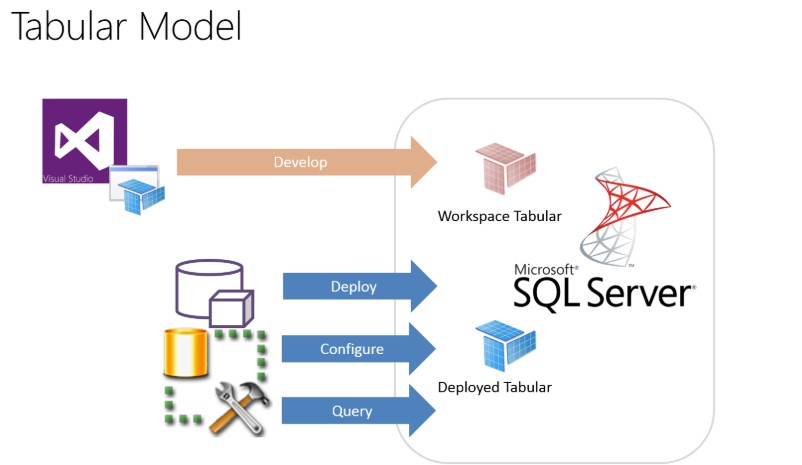
\includegraphics[width=12cm]{./Imagenes/img1} 
\end{center}


Sugerencias:
\begin{itemize}
	\item Primeramente, si ya se tiene una base de datos multidimensional, no se recomienda moverse a base de datos tabulares.
	\item El hardware requerido para un proyecto tabular es muy diferente al requerido por un proyecto multidimensional. Por la compresión de datos, requiere menos disco una modelo tabular, pero requiere mucha más memoria RAM porque todo lo usa en memoria. En general, se necesita un buen CPU y memoria.
	\item Los modelos tabulares consumen muchos recursos, por lo que se recomienda hacer pruebas del funcionamiento en un servidor de desarrollo y no en producción.
	\item Se puede tener un modelo tabular y uno multidimensional instalados en la misma máquina, pero no es recomendable hacerlo en producción.
\end{itemize}



\section{Ejemplo}
 
\section{Ventajas y Desventajas}

\subsection{Ventajas del Modelo Tabular}

\begin{itemize}
	\item Mucho más veloz en consultas.
	\item No requiere generar Aggregations (agregaciones) por lo que se simplifica el tiempo de procesamiento.
	\item Gracias al DAX (el lenguaje para acceder a los datos equivalente al MDX), tiene mayor flexibilidad para obtener información.
	\item Es intuitivo por lo que es mucho más rápido y fácil de entender e implementar.
	\item Se basa en modelos relacionales.
\end{itemize}

\subsection{Desventajas del Modelo Tabular}

\begin{itemize}
	\item Las particiones no se procesaban en paralelo si no secuencialmente, lo que hace que sea más lento el procesamiento.
	\item No se pueden usar multiples idiomas.
	\item Si son muchos datos tarda bastante en manejar configuraciones de diferentes particiones.
	\item El modelo tabular acapara demasiada memoria RAM y a su vez es dependiente de tal que afectará a otras aplicaciones.
\end{itemize}


\section{Diferencias}

\section{Conclusion}


%%
	
	%%
	%\linenumbers
	
	%% main text

	
	
	\newpage
	
		%ESTILO
	   \bibliography{BIBLIOGRAFIA}		%ARCHIVO .bib
	   \begin{thebibliography}{0}
              \bibitem{Ronald} 
 	    \bibitem{Angelo} 
                 \bibitem{Juan} http://tdan.com/data-warehouse-design-inmon-versus-kimball/20300
                  \bibitem{Jhordy} https://blog.bi-geek.com/arquitectura-comparativa-inmon-y-kimball/
                  \bibitem{Jhordy} https://churriwifi.wordpress.com/2010/04/19/15-2-ampliacion-conceptos-del-modelado-dimensional/
                    \bibitem{Brandon} https://twooctobers.com/blog/8-data-storytelling-concepts-with-examples/
                   \bibitem{Brandon}https://www.ucasal.edu.ar/htm/ingenieria/cuadernos/archivos/5-p56-rivadera-formateado.pdf

         \end{thebibliography}
	
\end{document}

%%
%% End of file `elsarticle-template-1-num.tex'.
